\chapter{Evaluation and Analysis Results}
The evaluation and analysis result chapter will provide all gathered and analyzed data from the different test runned in this thesis. The chapter is divided into different subsections for each test case. 
\section{General}
To be able to run analisis on the data gathered from the different packet capturings (pcaps) and present it in an understandable way, two different programs were used; Wireshark and VsCode with pyshark. Wireshark were used to extract numbers from the pcaps and Visual Studio Code (VS Code) was used to generate graphs from the pcaps for the events. Even tough it is possible to use Wireshark to generate the same graphs as with VS Code, VS Code was selected because it is easier to generate graphs that have the same measures to compare and they are more ascetically pleasing to look at.  
\\\\
When opening a pcap in Wireshark several statistics are possible to extract. By choosing the option of "Capture File Properties", several measures were extracted from here, such as packets, average packet size in bytes, bytes and average bytes per second. The numbers from each pcap were noted down and used as a value to compare both the events to each other and to the baseline. 
\\\\
In VS Code, python was used as the programming language as it includes the package pyshark which can be used towards tshark. Two scripts with a number of different if statements were used to generate the graphs depending on the users arguments passed to the script. The scripts only differs with if the user wants to display the graphs with number of packets or number of graphs on the y-axis. The code is displayed in its whole in appendix XXXX, and in pseudo code beneath in algorithm \ref{alg:GraphScript}. For each of the if statements, the same code block is included and are only shown once in algorithm \ref{alg:GraphScript}. The graphs are all generated with bytes and packets per 2 seconds. 

\begin{table}[!hbtp]
    \centering
    \caption{Overview of system arguments for scripts}
    \begin{adjustbox}{width=1\textwidth}
    \begin{tabular}{l|l|l|}
        \cline{2-3} & \textbf{Description} & \textbf{Values}\\ \hline
        \multicolumn{1}{|l|}{\textbf{Argument 1}} & Name of device & \begin{tabular}[c]{@{}l@{}}Netatmo\\ Mill\\ Nedis\end{tabular} \\ \hline
        \multicolumn{1}{|l|}{\textbf{Argument 2}} & Which packets to include & \begin{tabular}[c]{@{}l@{}}Inbound packets and bytes\\ Outbound packets and bytes\\ Inbound and outbound packets and bytes\end{tabular} \\ \hline
        \multicolumn{1}{|l|}{\textbf{Argument 3}} & Type of event & \begin{tabular}[c]{@{}l@{}}Cooking\\ Shower\\ Window\\ Weekend\\ Baseline\end{tabular} \\ \hline
        \multicolumn{1}{|l|}{\textbf{Argument 4}} & Maximum value for y-axis, in bytes or packets & "Numeric value" \\ \hline
    \end{tabular}
    \end{adjustbox}
    \label{tab:SystemArgumentsScripts}
\end{table}

\begin{algorithm}
\caption{Script for generating graphs}\label{alg:GraphScript}
\begin{algorithmic}
        \For{Each date of event} \Comment{Graph\_function start}
            \State Extract the packets from the right pcap
            \For{Each packet in pcap}
                \State Extract packet length in byte and time
                \State Display graph
            \EndFor
        \EndFor \Comment{Graph\_function end}\\
    \If{Argument 2 is Outbound}
        \If{Argument 1 is Netatmo}
            \State Set display filter to "wlan.sa == Netatmo MAC address"
        \ElsIf{Argument 1 is Mill}
            \State Set display filter to "wlan.sa == Mill MAC address"
        \ElsIf{Argument 1 is Nedis}
            \State Set display filter to "wlan.sa == Nedis MAC address"    
        \EndIf\\
    \ElsIf{Argument 2 is Inbound}
        \If{Argument 1 is Netatmo}
            \State Set display filter to "wlan.da == Netatmo MAC address"
        \ElsIf{Argument 1 is Mill}
            \State Set display filter to "wlan.da == Mill MAC address"
        \ElsIf{Argument 1 is Nedis}
            \State Set display filter to "wlan.da == Nedis MAC address"  
        \EndIf\\
    \If{Argument 3 is Shower} \Comment{Event if-cases start}
        \State Set the dates from when the events occured 
        \State Graph\_function
    \ElsIf{Argument 3 is Cooking}
        \State Set the dates from when the events occured 
        \State Graph\_function
    \ElsIf{Argument 3 is Window}
        \State Set the dates from when the events occured 
        \State Graph\_function
    \ElsIf{Argument 3 is Weekend}
        \State Set the dates from when the events occured 
        \State Graph\_function
    \ElsIf{Argument 3 is Baseline}
        \State Set the dates from when the events occured 
        \State Graph\_function
    \EndIf \Comment{Event if-cases end}
\end{algorithmic}
\end{algorithm}


\section{Baseline}
The capturing of baseline traffic were conducted over the course of 10 days in the same environment as the devices were when conducting the events. During the baseline, the devices have not been affected by the specific events, such as cooking, showering or window open in the same room as the devices resides. The baseline traffic will both be used to look at standard traffic from the devices and to compare this to the events in both graphs and calculations in sub chapter 5.3-5.5. The traffic from the capture file is encrypted on layer 2 (Wi-Fi) and therefore it is not possible to extract any values from the payload of the packets. 
\subsection{Netatmo Home Coach}
\textit{Figure \ref{fig:NetatmoBaselineTotalPackets}} and \textit{\ref{fig:NetatmoBaselineTotalBytes}} shows the graphs for Netatmo Home Coach from the baseline capturing from 6th of March 2023 to 15th of March 2023. 
\begin{figure} [H]
    \centering
    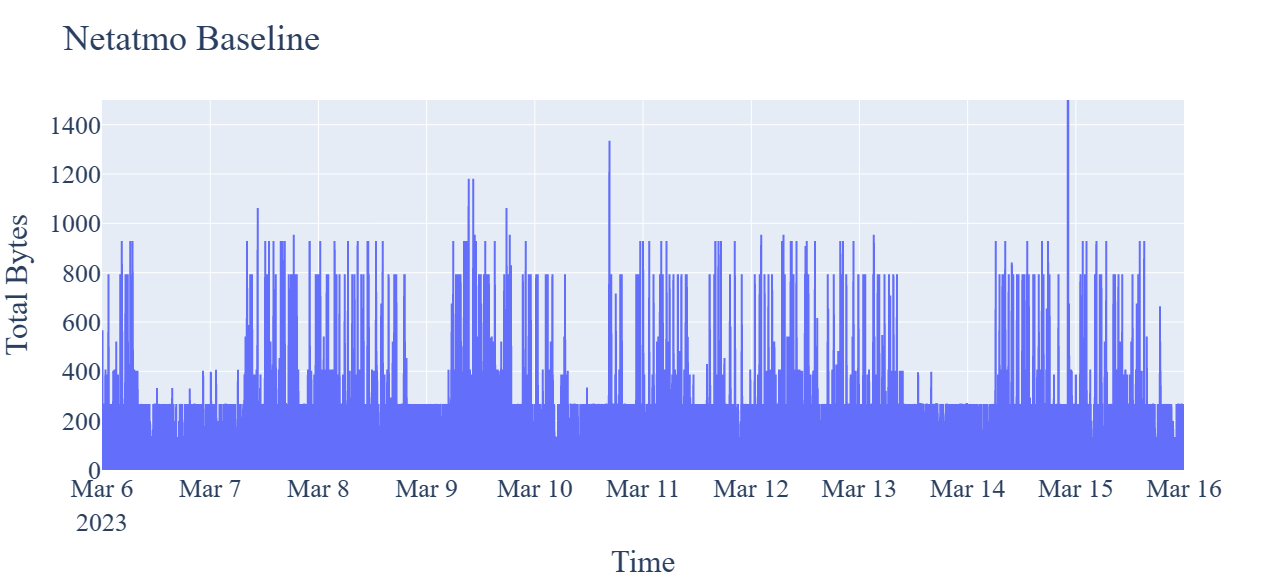
\includegraphics[scale=0.3]{figures/Netatmo_Baseline_TotalBytes.png}
    \caption{Netatmo Baseline Total Bytes}
    \label{fig:NetatmoBaselineTotalBytes}
\end{figure}

\begin{figure} [H]         
    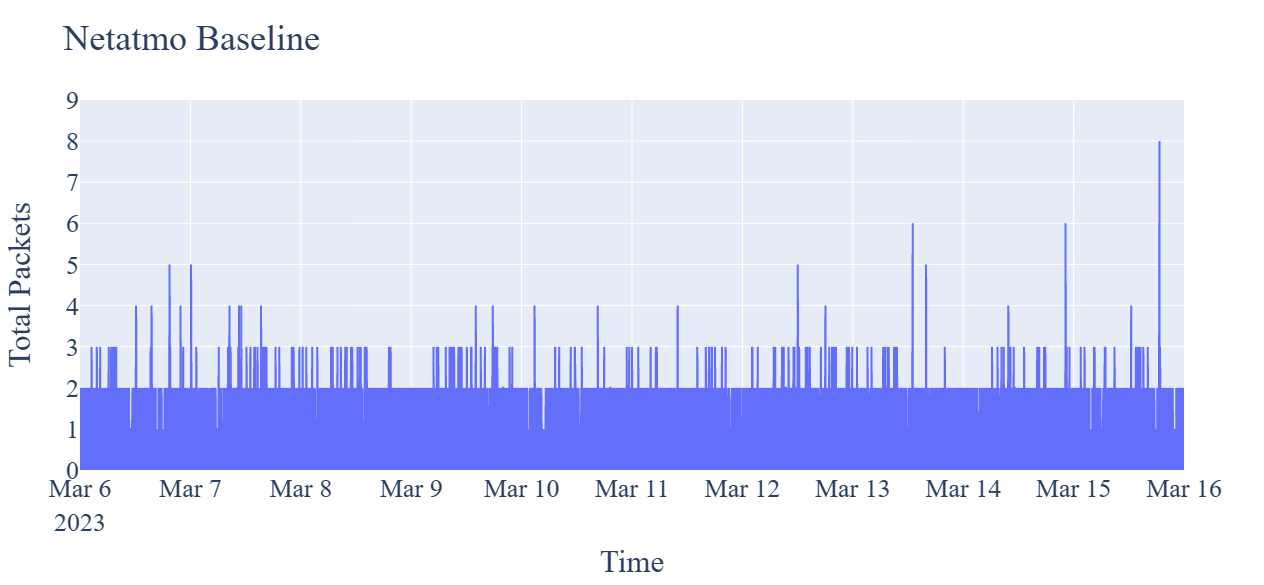
\includegraphics[scale=0.3]{figures/Netatmo_Baseline_TotalPackets.png}
    \caption{Netatmo Baseline Total Packets}
    \label{fig:NetatmoBaselineTotalPackets}
 \end{figure}

For the baseline graphs, it is possible to see that packets are sent continually at a rate of around 250 bytes per 2 seconds and 2 packets per 2 seconds. As these graphs shows the total packets and bytes sent and received, it can also be beneficial to look at what the graphs would look like if filtered on packets and bytes sent and packets and bytes received separately. 

\begin{figure}[H]
    \centering
    \begin{subfigure}[b]{0.7\textwidth}
        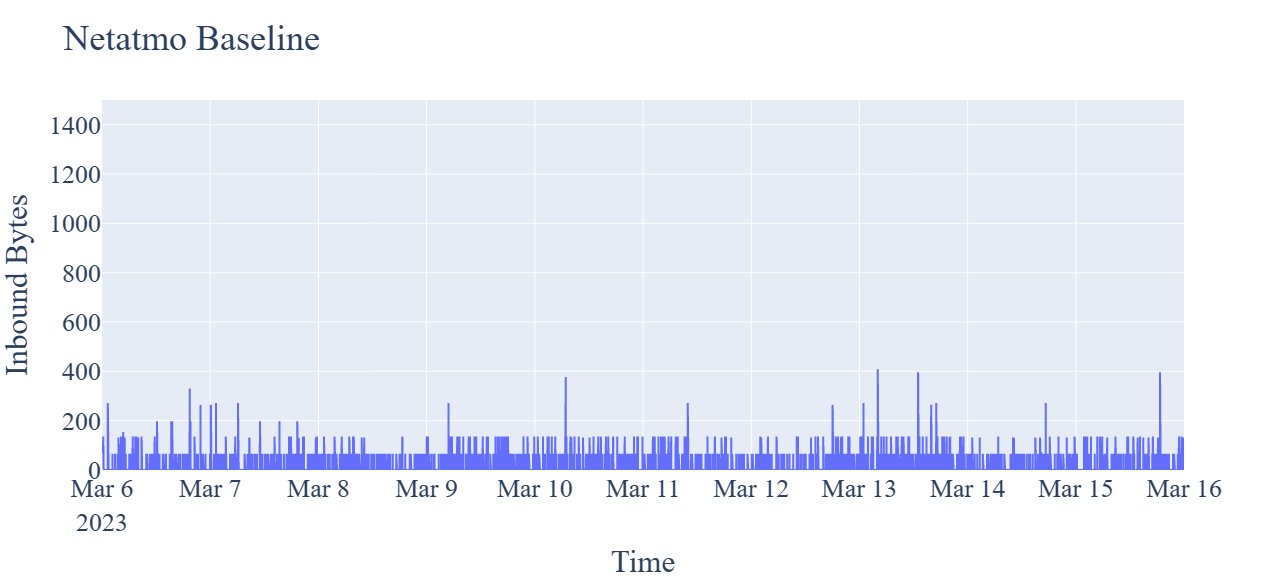
\includegraphics[width=\textwidth]{figures/Netatmo_Baseline_InboundBytes.png}
        \caption{Inbound Bytes}
        \label{fig:NetatmoBaselineInboundBytes}
    \end{subfigure}
    \begin{subfigure}[b]{0.7\textwidth}
        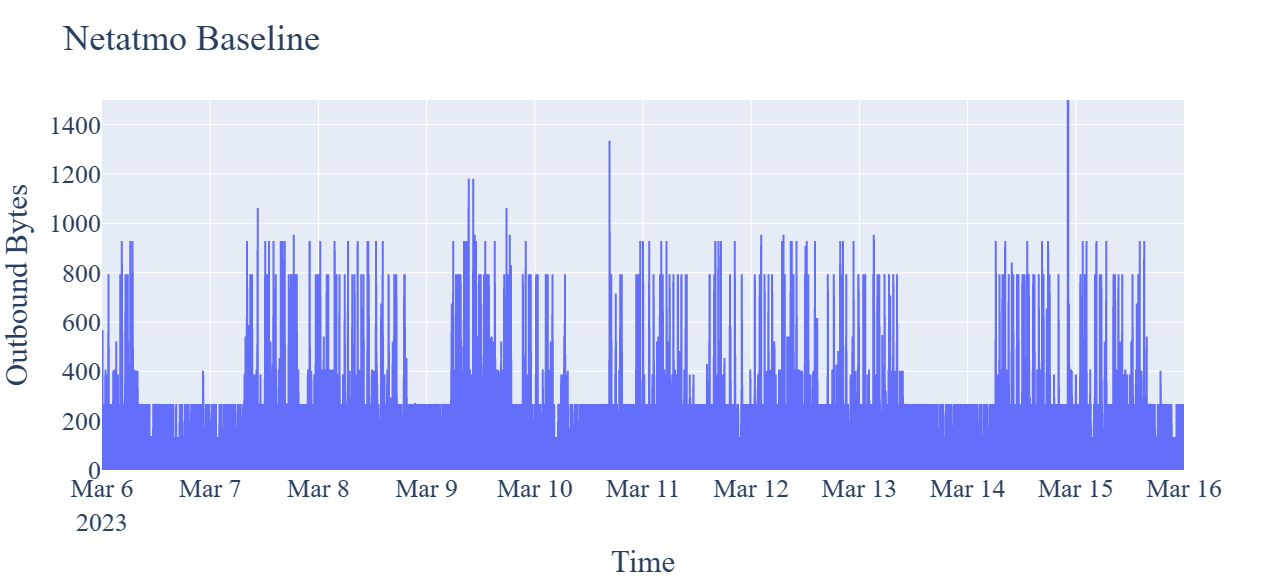
\includegraphics[width=\textwidth]{figures/Netatmo_Baseline_OutboundBytes.png}
        \caption{Outbound Bytes}
        \label{fig:NetatmoBaselineOutboundBytes}
    \end{subfigure}
    \caption{Netatmo Baseline Inbound and Outbound Bytes}
    \label{Fig:NetatmoBaselineOutandInboundBytes}
 \end{figure}

 \begin{figure}[H]
    \centering
    \begin{subfigure}[b]{0.7\textwidth}
        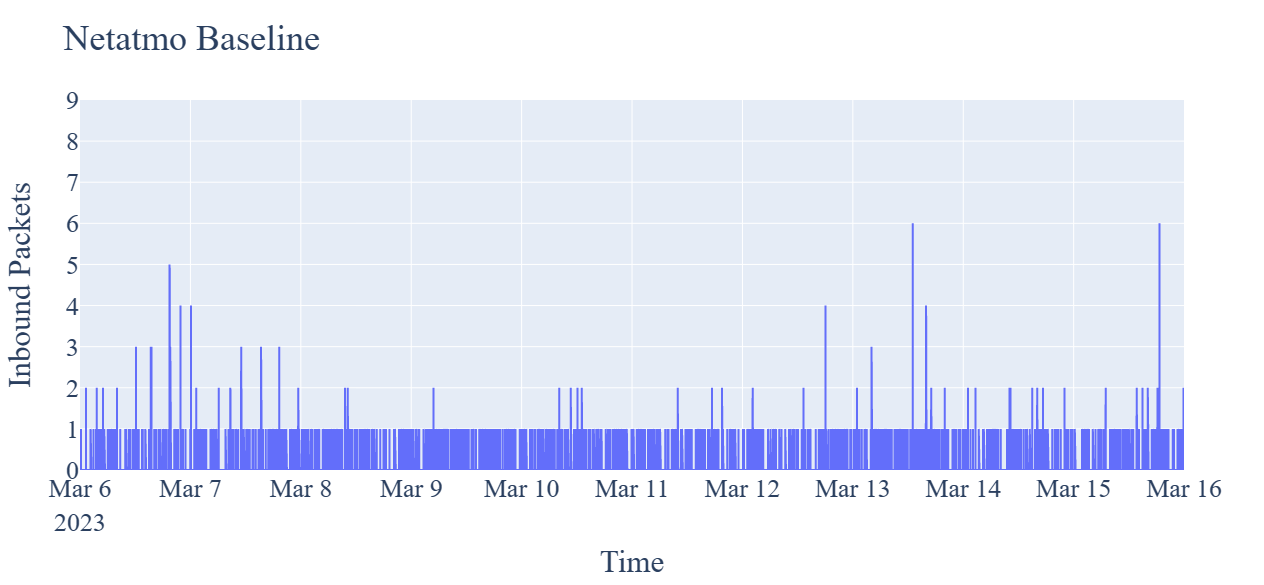
\includegraphics[width=\textwidth]{figures/Netatmo_Baseline_InboundPackets.png}
        \caption{Inbound Packets}
        \label{fig:NetatmoBaselineInboundPackets}
    \end{subfigure}
    \begin{subfigure}[b]{0.7\textwidth}
        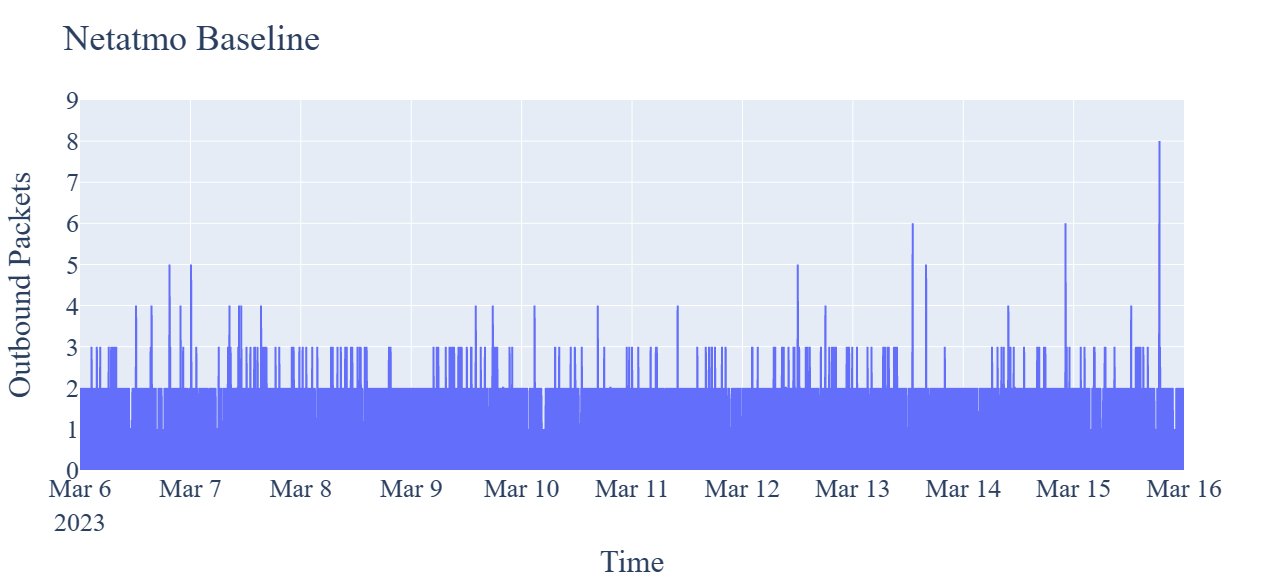
\includegraphics[width=\textwidth]{figures/Netatmo_Baseline_OutboundPackets.png}
        \caption{Outbound Packets}
        \label{fig:NetatmoBaselineOutboundPackets}
    \end{subfigure}
    \caption{Netatmo Baseline Inbound and Outbound Packets}
    \label{Fig:NetatmoBaselineOutandInboundPackets}
 \end{figure}
For the inbound and outbound bytes for Netatmo, \textit{figure \ref{Fig:NetatmoBaselineOutandInboundBytes}}, it is clear to see that the device sends a lot more bytes than it receives. The same pattern appears in \textit{figure \ref{Fig:NetatmoBaselineOutandInboundPackets}} for packets. Calculations made on the baseline traffic are presented in table \ref{tab:NetatmoBaselineCalculations}. 
\begin{table}[H]
    \caption{Calculations for Netatmo Baseline Capture}
    \centering
    \begin{tabular}{ll|l|}
        \cline{3-3}                                               &                               &             \textbf{Numbers} \\ \hline
        \multicolumn{1}{|c|}{\multirow{4}{*}{\textbf{Total}}}    & Packets              & 110,735         \\ \cline{2-3} 
        \multicolumn{1}{|c|}{}                                   & Bytes                & 14,959,396       \\ \cline{2-3} 
        \multicolumn{1}{|c|}{}                                   & Average bytes/second & 17               \\ \cline{2-3} 
        \multicolumn{1}{|c|}{}                                   & Average packet size  & 135 bytes        \\ \hline
        \multicolumn{1}{|l|}{\multirow{5}{*}{\textbf{Inbound}}}  & Packets              & 1,042            \\ \cline{2-3} 
        \multicolumn{1}{|l|}{}                                   & Bytes                & 83,446           \\ \cline{2-3} 
        \multicolumn{1}{|l|}{}                                   & Average bytes/second & 0                \\ \cline{2-3} 
        \multicolumn{1}{|l|}{}                                   & Average packet size  & 80 bytes          \\ \cline{2-3} 
        \multicolumn{1}{|l|}{}                                   & Biggest packet       & 377 bytes        \\ \hline
        \multicolumn{1}{|l|}{\multirow{5}{*}{\textbf{Outbound}}} & Packets              & 109,693          \\ \cline{2-3} 
        \multicolumn{1}{|l|}{}                                   & Bytes                & 14,875,950       \\ \cline{2-3} 
        \multicolumn{1}{|l|}{}                                   & Average bytes/second & 17               \\ \cline{2-3} 
        \multicolumn{1}{|l|}{}                                   & Average packet size  & 136 bytes         \\ \cline{2-3} 
        \multicolumn{1}{|l|}{}                                   & Biggest packet       & 1,150 bytes       \\ \hline
    \end{tabular}
    \label{tab:NetatmoBaselineCalculations}
\end{table}
When comparing the inbound(figure \ref{fig:NetatmoBaselineInboundBytes} and figures \ref{fig:NetatmoBaselineInboundPackets}) and outbound(figure \ref{fig:NetatmoBaselineOutboundBytes} and \ref{fig:NetatmoBaselineOutboundPackets}) graphs with the total graphs (figure \ref{fig:NetatmoBaselineTotalBytes} and figures \ref{fig:NetatmoBaselineTotalPackets}), the total graphs do not differ much from the outbound graphs, as they stand for the majority of packets and bytes. The same is numerically shown in table \ref{tab:NetatmoBaselineCalculations}, where over 99\% of the total packets are outbound traffic. Therefore, it will not be big differences in outbound and total graphs, so moving forward to the events only graphs for total traffic will be used to evaluate and analyze. The majority of packets sent from Netatmo are packets labeled "Data" with a size of 134 bytes, which makes up 98,3\% of the total packets from the capture file. 

\subsection{Mill Sense}
\textit{Figure \ref{fig:MillBaselineTotalPackets}} and \textit{\ref{fig:MillBaselineTotalBytes}} shows the graphs for Mill from the baseline capturing from 6th of March 2023 to 15th of March 2023. 
\begin{figure} [H]
    \centering
    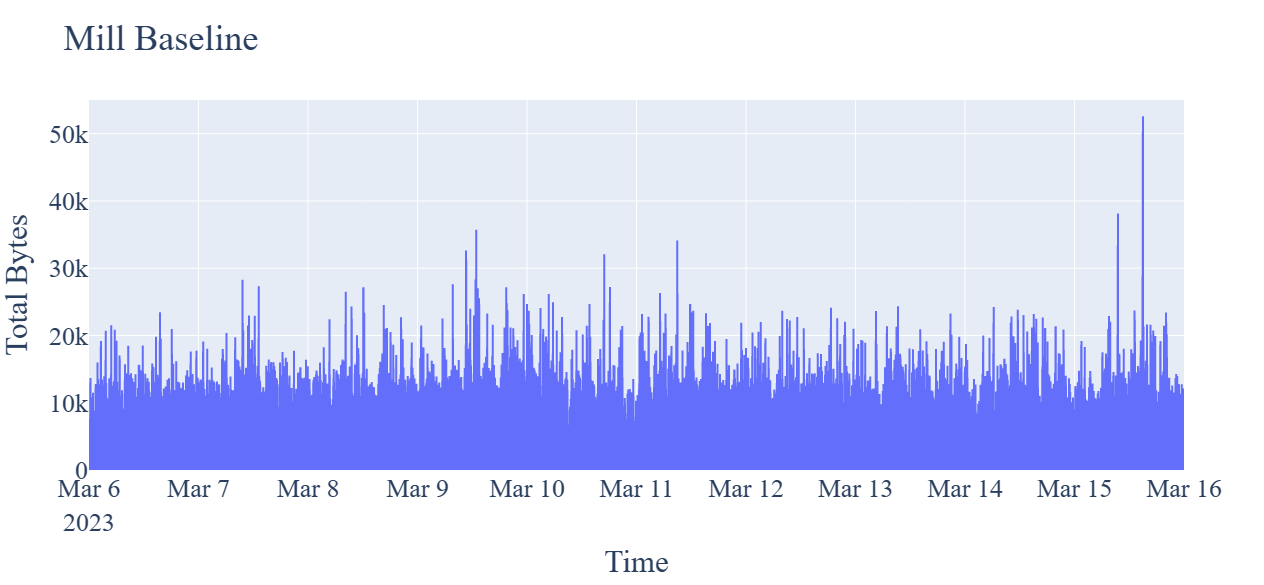
\includegraphics[scale=0.3]{figures/Mill_Baseline_TotalBytes.png}
    \caption{Mill Baseline Total Bytes}
    \label{fig:MillBaselineTotalBytes}
\end{figure}

\begin{figure} [H]         
    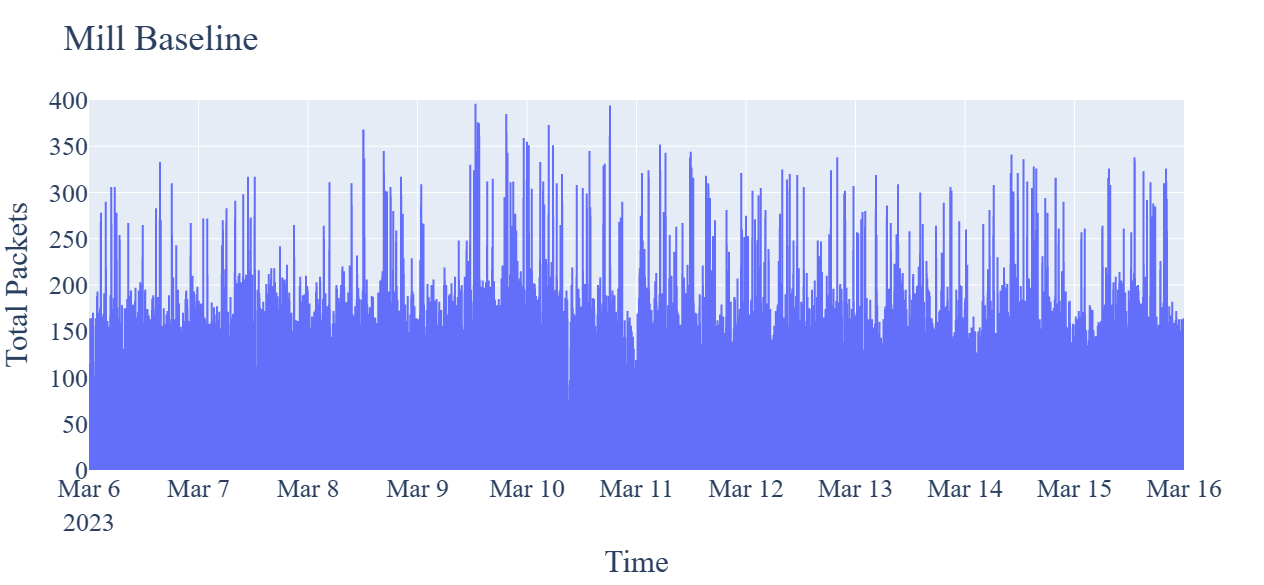
\includegraphics[scale=0.3]{figures/Mill_Baseline_TotalPackets.png}
    \caption{Mill Baseline Total Packets}
    \label{fig:MillBaselineTotalPackets}
 \end{figure}

The baseline traffic for Mill shows that the traffic varies a lot. As this device does not send live updates, but every minute, more spikes are included as it does not always send packets. 

\begin{figure}[H]
    \centering
    \begin{subfigure}[b]{0.7\textwidth}
        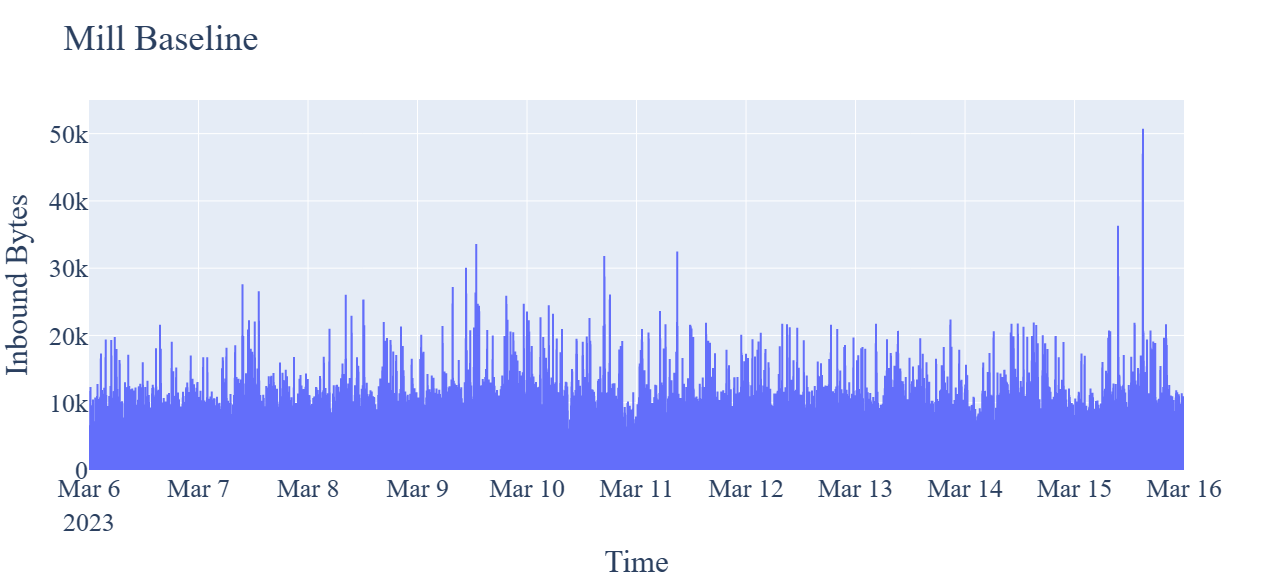
\includegraphics[width=\textwidth]{figures/Mill_Baseline_InboundBytes.png}
        \caption{Inbound Bytes}
        \label{fig:MillBaselineInboundBytes}
    \end{subfigure}
    \begin{subfigure}[b]{0.7\textwidth}
        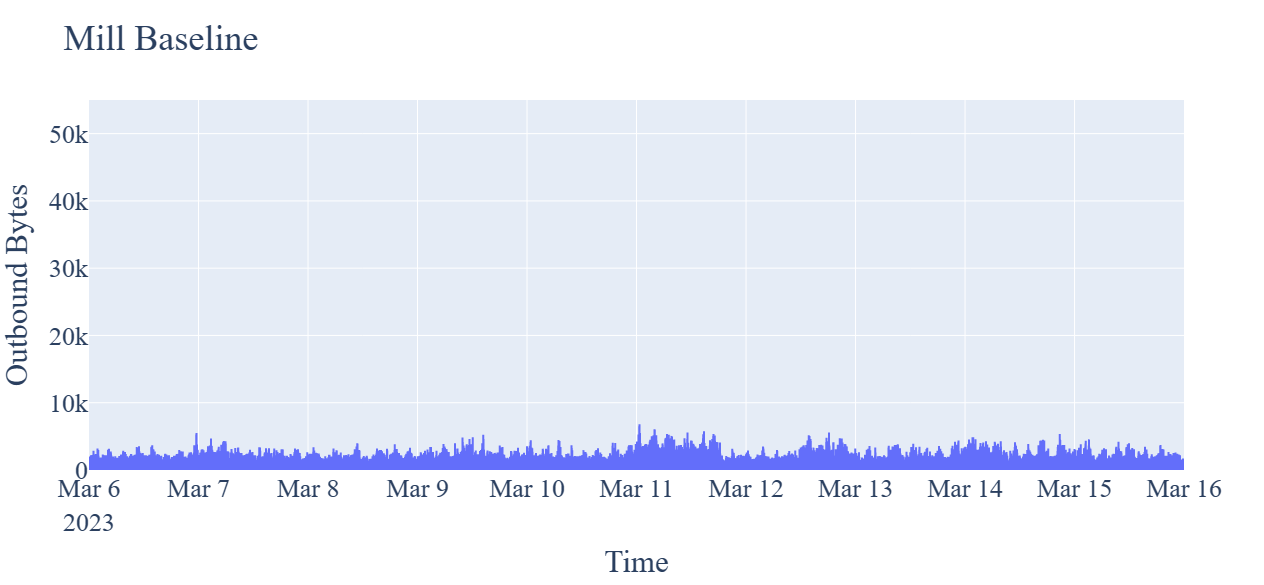
\includegraphics[width=\textwidth]{figures/Mill_Baseline_OutboundBytes.png}
        \caption{Outbound Bytes}
        \label{fig:MillBaselineOutboundBytes}
    \end{subfigure}
    \caption{Mill Baseline Inbound and Outbound Bytes}
    \label{Fig:MillBaselineOutandInboundBytes}
 \end{figure}

 \begin{figure}[H]
    \centering
    \begin{subfigure}[b]{0.7\textwidth}
        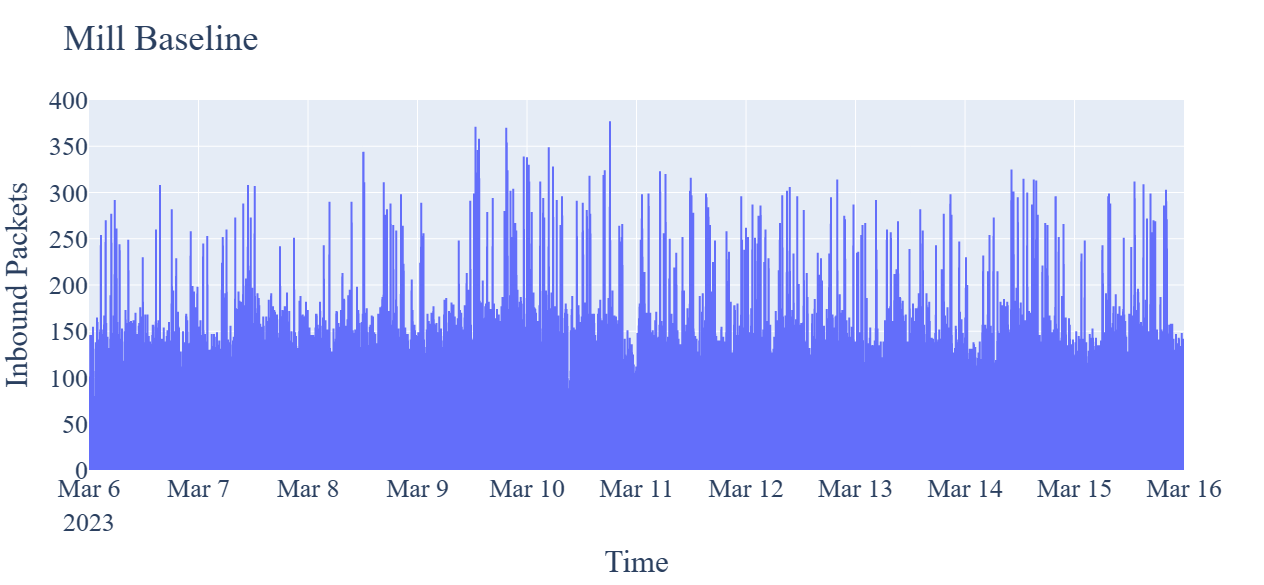
\includegraphics[width=\textwidth]{figures/Mill_Baseline_InboundPackets.png}
        \caption{Inbound Packets}
        \label{fig:MillBaselineInboundPackets}
    \end{subfigure}
    \begin{subfigure}[b]{0.7\textwidth}
        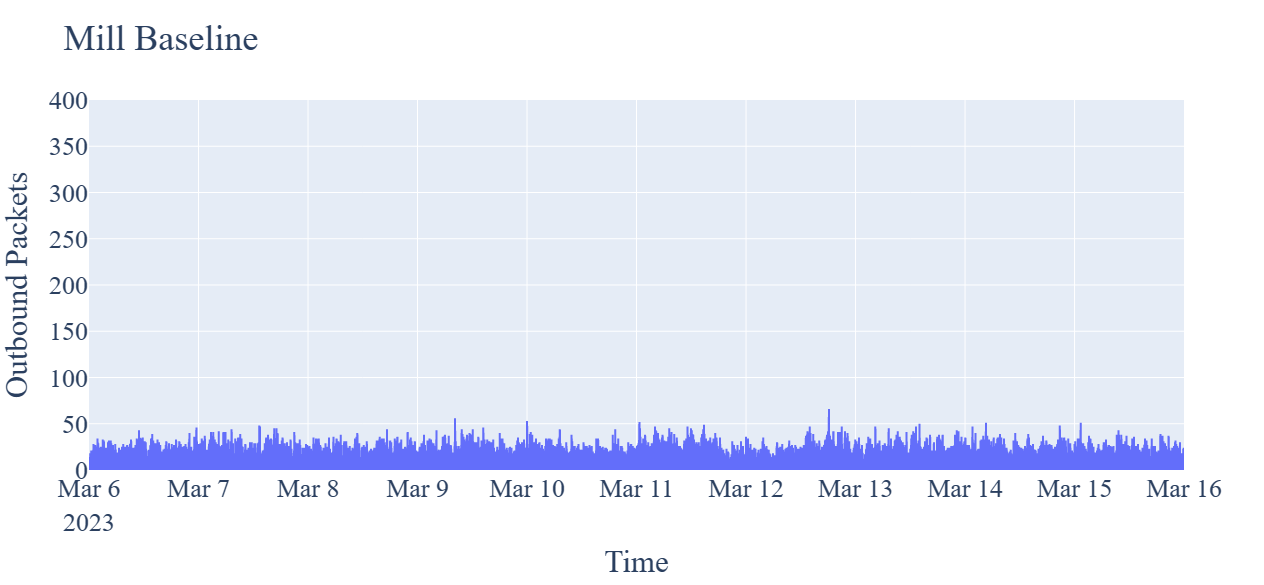
\includegraphics[width=\textwidth]{figures/Mill_Baseline_OutboundPackets.png}
        \caption{Outbound Packets}
        \label{fig:MillBaselineOutboundPackets}
    \end{subfigure}
    \caption{Mill Baseline Inbound and Outbound Packets}
    \label{Fig:MillBaselineOutandInboundPackets}
 \end{figure}

\begin{table}[H]
    \caption{Calculations for Mill Baseline Capture}
    \centering
    \begin{tabular}{ll|l|}
        \cline{3-3}                                               &                               &             \textbf{Numbers} \\ \hline
        \multicolumn{1}{|c|}{\multirow{4}{*}{\textbf{Total}}}    & Packets              & 1,236,753         \\ \cline{2-3} 
        \multicolumn{1}{|c|}{}                                   & Bytes                & 129,253,290       \\ \cline{2-3} 
        \multicolumn{1}{|c|}{}                                   & Average bytes/second & 149              \\ \cline{2-3} 
        \multicolumn{1}{|c|}{}                                   & Average packet size  & 105 bytes        \\ \hline
        \multicolumn{1}{|l|}{\multirow{5}{*}{\textbf{Inbound}}}  & Packets              & 942,112           \\ \cline{2-3} 
        \multicolumn{1}{|l|}{}                                   & Bytes                & 95,458,773        \\ \cline{2-3} 
        \multicolumn{1}{|l|}{}                                   & Average bytes/second & 110              \\ \cline{2-3} 
        \multicolumn{1}{|l|}{}                                   & Average packet size  & 101 bytes         \\ \cline{2-3} 
        \multicolumn{1}{|l|}{}                                   & Biggest packet       & 1593 bytes        \\ \hline
        \multicolumn{1}{|l|}{\multirow{5}{*}{\textbf{Outbound}}} & Packets              & 294,640          \\ \cline{2-3} 
        \multicolumn{1}{|l|}{}                                   & Bytes                & 33,794,517       \\ \cline{2-3} 
        \multicolumn{1}{|l|}{}                                   & Average bytes/second & 39               \\ \cline{2-3} 
        \multicolumn{1}{|l|}{}                                   & Average packet size  & 115 bytes         \\ \cline{2-3} 
        \multicolumn{1}{|l|}{}                                   & Biggest packet       & 456 bytes       \\ \hline
    \end{tabular}
    \label{tab:MillBaselineCalculations}
\end{table}


\subsection{Nedis}
\textit{Figure \ref{fig:NedisBaselineTotalPackets}} and \textit{\ref{fig:NedisBaselineTotalBytes}} shows the graphs for Nedis from the baseline capturing from 6th of March 2023 to 15th of March 2023. 
\begin{figure} [H]
    \centering
    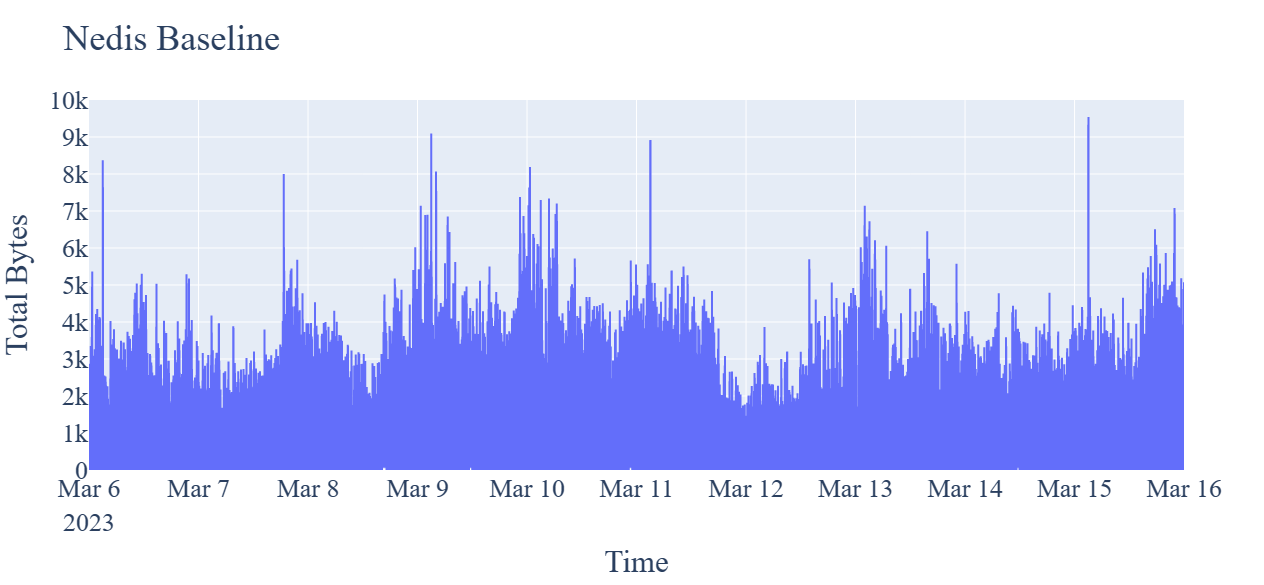
\includegraphics[scale=0.3]{figures/Nedis_Baseline_TotalBytes.png}
    \caption{Nedis Baseline Total Bytes}
    \label{fig:NedisBaselineTotalBytes}
\end{figure}

\begin{figure} [H]         
    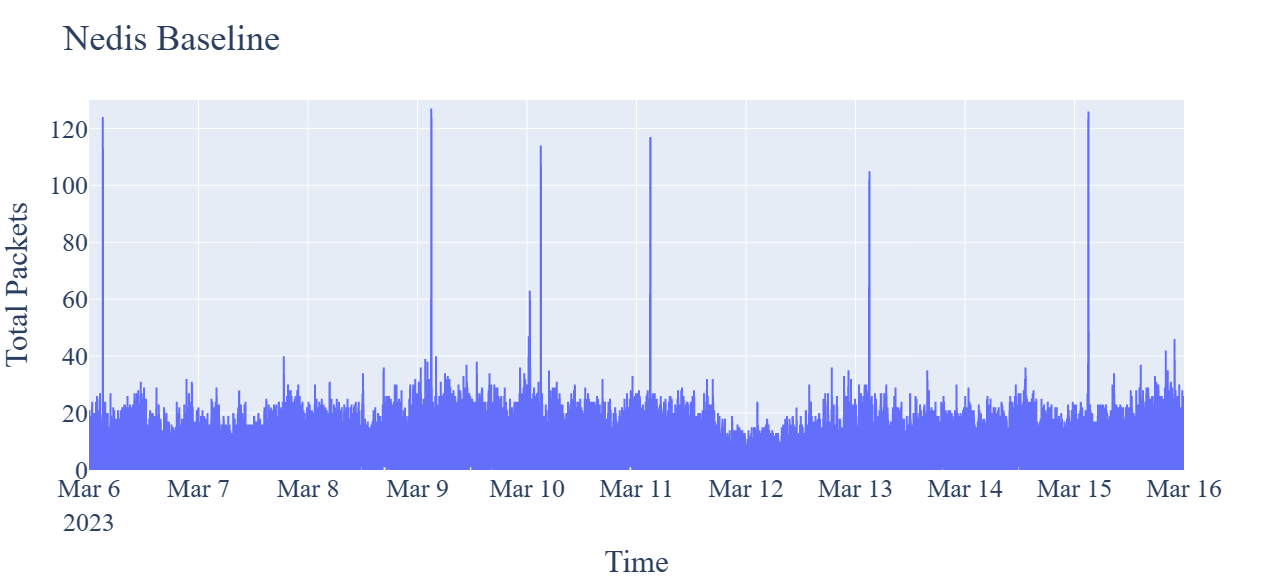
\includegraphics[scale=0.3]{figures/Nedis_Baseline_TotalPackets.png}
    \caption{Nedis Baseline Total Packets}
    \label{fig:NedisBaselineTotalPackets}
 \end{figure}



\begin{figure}[H]
    \centering
    \begin{subfigure}[b]{0.7\textwidth}
        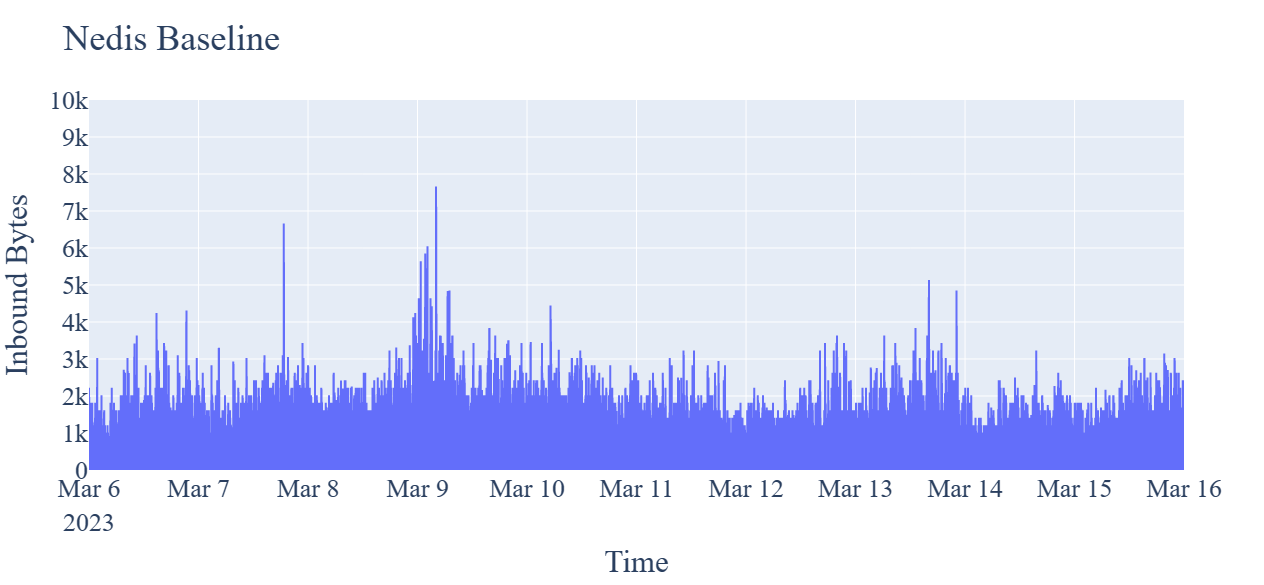
\includegraphics[width=\textwidth]{figures/Nedis_Baseline_InboundBytes.png}
        \caption{Inbound Bytes}
        \label{fig:NedisBaselineInboundBytes}
    \end{subfigure}
    \begin{subfigure}[b]{0.7\textwidth}
        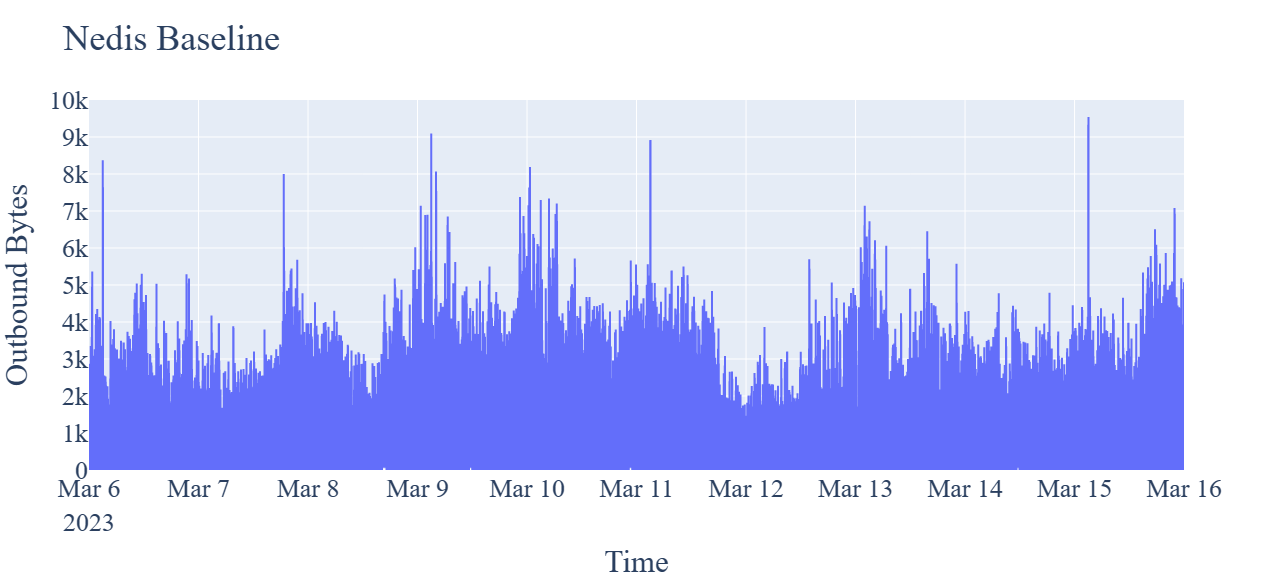
\includegraphics[width=\textwidth]{figures/Nedis_Baseline_OutboundBytes.png}
        \caption{Outbound Bytes}
        \label{fig:NedisBaselineOutboundBytes}
    \end{subfigure}
    \caption{Nedis Baseline Inbound and Outbound Bytes}
    \label{Fig:NedisBaselineOutandInboundBytes}
 \end{figure}

 \begin{figure}[H]
    \centering
    \begin{subfigure}[b]{0.7\textwidth}
        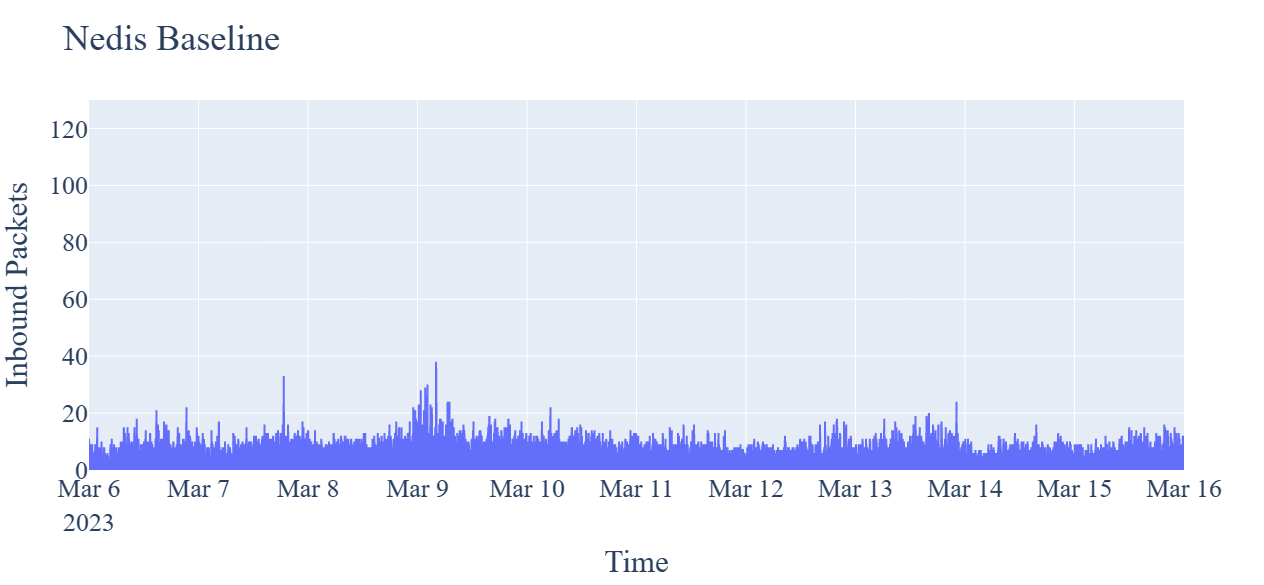
\includegraphics[width=\textwidth]{figures/Nedis_Baseline_InboundPackets.png}
        \caption{Inbound Packets}
        \label{fig:NedisBaselineInboundPackets}
    \end{subfigure}
    \begin{subfigure}[b]{0.7\textwidth}
        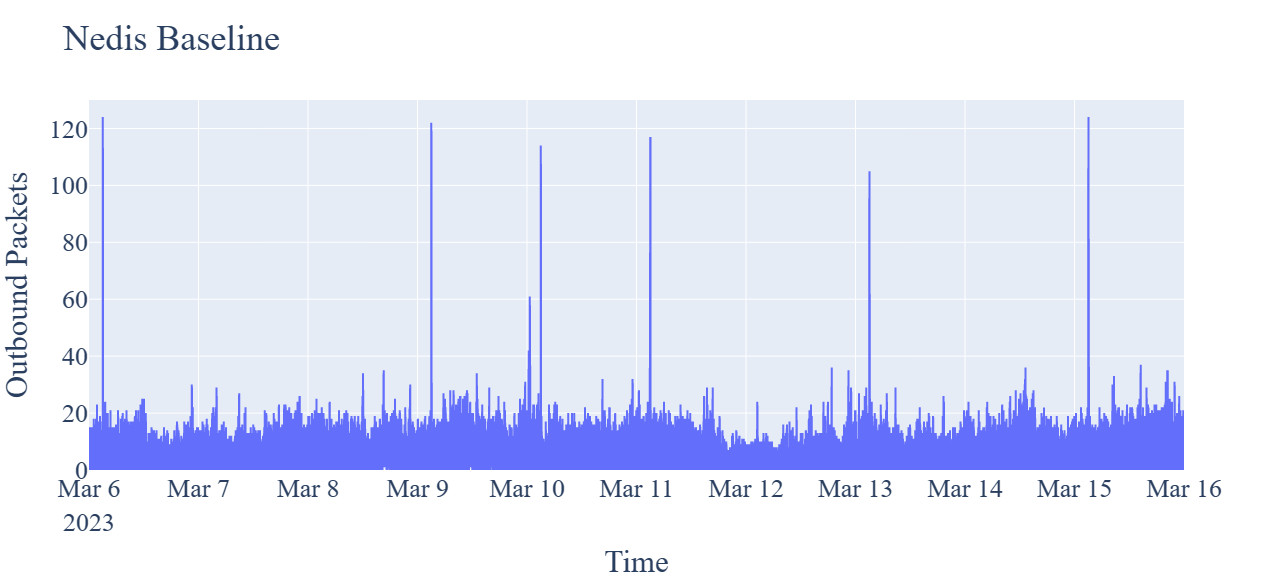
\includegraphics[width=\textwidth]{figures/Nedis_Baseline_OutboundPackets.png}
        \caption{Outbound Packets}
        \label{fig:NedisBaselineOutboundPackets}
    \end{subfigure}
    \caption{Nedis Baseline Inbound and Outbound Packets}
    \label{Fig:NedisBaselineOutandInboundPackets}
 \end{figure}
 
\begin{table}[H]
    \caption{Calculations for Nedis Baseline Capture}
    \centering
    \begin{tabular}{ll|l|}
        \cline{3-3}                                               &                               &             \textbf{Numbers} \\ \hline
        \multicolumn{1}{|c|}{\multirow{4}{*}{\textbf{Total}}}    & Packets              & 2,428,701         \\ \cline{2-3} 
        \multicolumn{1}{|c|}{}                                   & Bytes                & 295,022,494       \\ \cline{2-3} 
        \multicolumn{1}{|c|}{}                                   & Average bytes/second & 341               \\ \cline{2-3} 
        \multicolumn{1}{|c|}{}                                   & Average packet size  & 121 bytes        \\ \hline
        \multicolumn{1}{|l|}{\multirow{5}{*}{\textbf{Inbound}}}  & Packets              & 451,495           \\ \cline{2-3} 
        \multicolumn{1}{|l|}{}                                   & Bytes                & 88,595,049        \\ \cline{2-3} 
        \multicolumn{1}{|l|}{}                                   & Average bytes/second & 102                \\ \cline{2-3} 
        \multicolumn{1}{|l|}{}                                   & Average packet size  & 196 bytes         \\ \cline{2-3} 
        \multicolumn{1}{|l|}{}                                   & Biggest packet       & 522 bytes        \\ \hline
        \multicolumn{1}{|l|}{\multirow{5}{*}{\textbf{Outbound}}} & Packets              & 1,977,206         \\ \cline{2-3} 
        \multicolumn{1}{|l|}{}                                   & Bytes                & 206,427,445      \\ \cline{2-3} 
        \multicolumn{1}{|l|}{}                                   & Average bytes/second & 238               \\ \cline{2-3} 
        \multicolumn{1}{|l|}{}                                   & Average packet size  & 104 bytes         \\ \cline{2-3} 
        \multicolumn{1}{|l|}{}                                   & Biggest packet       & 485 bytes       \\ \hline
    \end{tabular}
    \label{tab:NedisBaselineCalculations}
\end{table} 


\section{Test Case 1: Cooking}
This chapter presents the results and analysis conducted on Test Case 1: Cooking.
\subsection{General}
The cooking events are 15 in total and are presented in table \ref{tab:CookingDates}. Every device have the same dates for this event. 
\begin{table}[!hbtp]
    \centering
    \caption{Date and time for Test Case 1: Cooking Events}
    \begin{adjustbox}{width=1\textwidth}
            \begin{tabular}{l|l|l|l|l|l|l|l|l|l|l|l|l|l|l|l|}
            \cline{2-16} 
            & 08.01 & 09.01 & 10.01 & 11.01 & 12.01 & 16.01 & 18.01 & 19.01 & 24.01 & 25.01 & 26.01 & 30.01 & 31.01 & 01.02 & 02.02 \\
            \hline
            \multicolumn{1}{|l|}{Started event}  & 15:58 & 15:59 & 16:01 & 16:05 & 16:10 & 16:02 & 16:04 & 16:01 & 15:57 & 16:02 & 16:01 & 16:01 & 16:01 & 16:02 & 16:02 \\ 
            \hline
            \multicolumn{1}{|l|}{Finished event} & 16:22 & 16:21 & 16:27 & 16:37 & 16:28 & 16:25 & 16:25 & 16:18 & 16:20 & 16:13 & 16:25 & 16:19 & 16:21 & 16:22 & 16:22 \\ 
            \hline
            \end{tabular}
    \end{adjustbox}
    \label{tab:CookingDates}
\end{table}
\FloatBarrier

To be able to look even further into differences from when the devices are in an environment when an event is ongoing and when it is in the same environment, but without any event ongoing, graphs and calculations from the baseline traffic are used to compare. To choose a time for the baseline traffic, all start values from the actual events in table XXX are used to calculate an average value for starting time. The same applies to end time. 


\subsection{Netatmo Home Coach}
\subsection{Mill Sense}
\subsection{Nedis}

\section{Test Case 2: Showering}
This chapter presents the results and analysis conducted on Test Case 2: Showering. 
\subsection{General}
\begin{table}[!hbtp]
    \centering
    \caption{Date and time for Test Case 2: Showering events}
    \begin{adjustbox}{width=1\textwidth} 
        \begin{tabular}{l|l|l|l|l|l|l|l|l|l|l|l|l|l|l|l|}
            \cline{2-16}
                & 08.01 & 09.01 & 11.01 & 12.01 & 16.01 & 18.01 & 19.01 & 23.01 & 24.01 & 26.01 & 30.01 & 31.01 & 01.02 & 02.02 & 06.02 \\ \hline
            \multicolumn{1}{|l|}{Started event}  & 19:59 & 20:14 & 20:01 & 19:59 & 20:12 & 20:02 & 20:00 & 20:00 & 20:03 & 20:03 & 20:00 & 20:01 & 20:00 & 20:00 & 20:00 \\ \hline
            \multicolumn{1}{|l|}{Finished event} & 20:14 & 20:34 & 20:17 & 20:21 & 20:31 & 20:19 & 20:16 & 20:21 & 20:19 & 20:19 & 20:18 & 20:17 & 20:16 & 20:17 & 20:17 \\ \hline
        \end{tabular}
    \end{adjustbox}
    \label{tab:ShoweringDates}
\end{table}

\subsection{Netatmo Home Coach}
\subsection{Mill Sense}
\subsection{Nedis}

\section{Test Case 3: Window Open}
This chapter presents the results and analysis conducted on Test Case 3: Window Open. 
\subsection{General}
\begin{table}[!hbtp]
    \centering
    \caption{Date and time for Test Case 3: Window Open events}
    \begin{adjustbox}{width=1\textwidth} 
            \begin{tabular}{l|l|l|l|l|l|l|l|l|l|l|l|l|l|l|l|}
                \cline{2-16}
                & 08.01 & 09.01 & 10.01 & 11.01 & 12.01 & 16.01 & 18.01 & 19.01 & 23.01 & 24.01 & 25.01 & 30.01 & 31.01 & 01.02 & 02.02 \\ \hline
                \multicolumn{1}{|l|}{Started event}  & 23:00 & 23:00 & 23:00 & 22:50 & 23:00 & 23:10 & 23:15 & 23:02 & 22:59 & 22:59 & 22:59 & 23:00 & 22:59 & 22:59 & 22:59 \\ \hline
                \multicolumn{1}{|l|}{Finished event} & 07:00 & 07:00 & 07:00 & 07:00 & 07:00 & 06:56 & 07:09 & 06:59 & 06:55 & 06:57 & 06:55 & 06:56 & 07:00 & 06:59 & 06:59 \\ \hline
            \end{tabular}
    \end{adjustbox}
    \label{tab:WindowDates}
\end{table}
\subsection{Netatmo Home Coach}
\subsection{Mill Sense}
\subsection{Nedis}

\section{Test Case 4: Weekends}
This chapter presents the results and analysis conducted on Test Case 4: Weekends. 
\subsection{General}
Test Case 4: Weekends are tested over the course of 14 different weekends. 7 weekends when the environment was occupied and 7 when the environment were not occupied. The different dates are described in table \ref{tab:WeekendDates}. 
\begin{table}[!hbtp]
    \centering
    \caption{Dates for Test Case 4: Weekends}
    \begin{adjustbox}{width=0.5\textwidth} 
        \begin{tabular}{l|l|}
            \cline{2-2} & \textbf{Dates}\\ \hline
            \multicolumn{1}{|l|}{\textbf{Occupied}} & \begin{tabular}[c]{@{}l@{}}13.01.2023-15.01.2023\\ 27.01.2023-29.01.2023\\ 03.02.2023-05.02.2023\\ 17.02.2023-19.02.2023\\ 10.03.2023-12.03.2023\\ 28.03.2023-30.03.2023\\ 31.03.2023-01.04.2023\end{tabular} \\ \hline
            \multicolumn{1}{|l|}{\textbf{Not occupied}} & \begin{tabular}[c]{@{}l@{}}23.12.2022-25.12.2022\\ 30.12.2022-01.01.2023\\ 20.01.2023-22.01.2023\\ 10.02.2023-12.02.2023\\ 24.02.2023-26.02.2023\\ 03.03.2023-05.03.2023\\ 17.03.2023-19.03.2023\end{tabular} \\ \hline
        \end{tabular}
    \end{adjustbox}
    \label{tab:WeekendDates}
\end{table}

\subsection{Netatmo Home Coach}
\subsection{Mill Sense}
\subsection{Nedis}